\documentclass[11pt]{article}
\usepackage{enumerate}
\usepackage{amsfonts}
\usepackage{graphicx}
\usepackage{listings}
\usepackage{float}
\usepackage{tikz}
\usepackage{subcaption}
\pagestyle{empty} \setlength{\parindent}{0mm}
\addtolength{\topmargin}{-0.5in} \setlength{\textheight}{9.5in}
\addtolength{\textwidth}{0.5in} \addtolength{\oddsidemargin}{-0.5in}

\begin{document}

\begin{center}
\textbf{Logan Sims \\ CSCI 402 \\ Homework 2  }
\end{center}

\begin{enumerate}[1.]
\item
  \begin{enumerate}[a.]
  \item
  The state space for this problem can be represented as a four-tuple in the following way:\\\\
  N: The set of states, a state a configuration of the game board.\\
  A: The set of arcs that represent actions taken to go from one unique state to the next.\\
  S: The start state.\\
  GD: The goal state.\\
  
  Actions in this state space will be represented as moving the blank, similar to the 8-puzzle example. The two legal moves now become://
  \begin{enumerate}[i.]
  \item Exchange blank with a tile to the left or right of it for a cost of one.
  \item Exchange the blank with a title 2 or 3 tiles away. This has a cost of the blank from the exchange tile minus one. 
  \end{enumerate}
  
  A Breadth-first search could be used to explore all states in this space. It would be possible for a state to be discovered multiple times causing loops. However by storing these space as a tree loops would not be a problem. Also all white tiles will be treated as the same and all black tiles the same. What this means is swapping two white or two black tiles creates the same state as before. Since the arcs of the tree represent actions that lead to different states the search space will not be filled with duplicate spaces. 
  
  \item
  A heuristic for this problem could be counting the number of white tiles that are to the right of the black tiles. By counting tiles and making moves that help to decrease the number of incorrect tile placements this heuristic can find a solution. Since the goal state requires all white tiles be on the left the program would choose paths that attempt to get closer to the goal state.\\
  
  By using the approach to determine admissibility similar to the one presented in the textbook, this heuristic is admissible because the number of tiles out of place is less than or equal to the number of moves required to get to the goal state.\\
  
  This heuristic is monotonic. The max h(n) can equal is three. This is also the value at the start state. Once the algorithm begins working if it finds a state with h(n) = 1 then for the algorithm to not be monotonic this state must cost at most 1 to get two. However that implies getting one black tile around 2 white tiles with a cost of one. This is impossible thus the heuristic is monotonic. \\
  
  The heuristic is more informed than a breadth-first search because it is able to prioritize paths that could lead to a goal state. Breadth-first search simple performs an unbiased exploration of the state space. However, the algorithm can only ever assume a cost of 3 or less. Many games will take more than 3 moves to complete. My conclusion is that there are other heuristics that could be more informed than mine.\\
  \end{enumerate}

\item
  \begin{enumerate}[a.]
  \item The following 8-puzzle start state demonstrates a reversal. The solution to this puzzle requires 11 moves to solve.

\begin{figure}[htbp]
    \centering
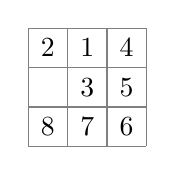
\begin{tikzpicture}
\draw[step=0.5cm,color=gray] (-1,-.5) grid (.5,1);
\node at (-0.75,+0.75) {2};
\node at (-0.25,+0.75) {1};
\node at (+0.25,+0.75) {4};

\node at (-0.75,+0.25) {};
\node at (-0.25,+0.25) {3};
\node at (+0.25,+0.25) {5};

\node at (-0.75,-0.25) {8};
\node at (-0.25,-0.25) {7};
\node at (+0.25,-0.25) {6};
\end{tikzpicture}
\end{figure}


\begin{center} 
\begin{tabular}{| l | l | l |} 
\hline Number & \textbf{Heuristic} & \textbf{Estimate}\\
\hline 1 & Tiles out of place. & 8\\ 
\hline 2 & Sum of distance out of place. &  9\\ 
\hline 3 & 2x number of direct reversals. & 4  \\ 
\hline 4 & Sum dist. out of place plus 2x num. reversals. & 11 \\
\hline 
\end{tabular} 
\end{center} 

Based on the example above the 4th heuristic is the exact cost making it the most accurate.\\
  \item
  Since it was established in the text that the 2nd heuristic was the most informed compared to the 1st and 3rd there only needs to be a comparison of the 2nd and 4th. Seeing as how the 4th takes into account that reversals are costly it will in fact prune the state space more efficiently that the 2nd heuristic. This makes the 4th heuristic the most informed. This also holds true in the \\
  \item
  The heuristics one, two, and 4, are monotonic because the difference between the heuristic cost of a node and any of it's children is less than or equal to the actual cost t0 get to the children. The third heuristic is not. Say there is a one tile reversal at state n1, h(n1) = 2. Now a child state, say n2, could cause the two tiles to no longer be next to each other. Now h(n2) = 0; the difference between these two states is 2, yet the cost was only 1. This shows that the third heuristic is not monotonic.  
  \item
  The first three are bounded from above. For the first heuristic it is because the number of tiles out of place is less than or equal to the number of moves require to put them in place. The same is true for the second heuristic because the distances are less than or equal to the moves required. Using a multiplier of two on the number of reversals is also admissible. This is because it requires many more moves to undo a reversal than the multiplier can add up to. The forth heuristic is also admissibly because it estimates the number of moves required to complete the puzzle.\\
  \end{enumerate}
\end{enumerate}
\end{document}